% Practice Test 17 — Indiana Edition
% Questions: 30 (19 MC + 11 SA)
% Generated by scripts/generate_practice_tests.py

\begin{practiceQuestion}{1-3-q27}{gmc}
\begin{questionText}
The table below shows a proportional relationship between gallons of gas and miles driven. What is $k$ and what does it mean?

\begin{center}
\begin{tabular}{|c|c|}
\hline
\textbf{Gallons ($x$)} & \textbf{Miles ($y$)} \\ \hline
$2$ & $54$ \\ \hline
$5$ & $135$ \\ \hline
$8$ & $216$ \\ \hline
\end{tabular}
\end{center}
\end{questionText}
\choiceA{$k = 2$; uses $2$ gallons per trip}
\choiceB{$k = 27$; drives $27$ miles per gallon}
\choiceC{$k = 54$; drives $54$ miles on $2$ gallons}
\choiceD{$k = 135$; drives $135$ miles on $5$ gallons}
\correctAnswer{B}
\explanation{$k = \frac{54}{2} = 27$, $\frac{135}{5} = 27$, $\frac{216}{8} = 27$. The car gets $27$ miles per gallon.}
\end{practiceQuestion}

\begin{practiceQuestion}{1-5-q29}{gsa}
\begin{questionText}
The graph below shows the number of birdhouses a carpenter can build over time. What is the unit rate, and how many birdhouses can be built in $10$ hours?

\begin{center}
\begin{tikzpicture}[scale=0.7]
  \draw[step=1,gray!20,thin] (0,0) grid (7,7);
  \draw[thick,->] (0,0) -- (7.5,0) node[right]{\small Hours};
  \draw[thick,->] (0,0) -- (0,7.5) node[above]{\small Birdhouses};
  \foreach \x in {1,...,7} \draw (\x,0.07) -- (\x,-0.07) node[below]{\tiny \x};
  \foreach \y in {1,...,7} \draw (0.07,\y) -- (-0.07,\y) node[left]{\tiny \y};
  \draw[thick,funBlue] (0,0) -- (7,5.25);
  \fill[funBlue] (0,0) circle (2.5pt);
  \fill[funBlue] (4,3) circle (2.5pt) node[above left]{\small $(4, 3)$};
\end{tikzpicture}
\end{center}
\end{questionText}
\correctAnswer{$0.75$ birdhouses per hour; $7.5$ birdhouses in $10$ hours}
\explanation{$k = \frac{3}{4} = 0.75$. In $10$ hours: $0.75 \times 10 = 7.5$ birdhouses.}
\end{practiceQuestion}

\begin{practiceQuestion}{1-6-q30}{gsa}
\begin{questionText}
The table shows how many batches of muffins a bakery can make and the total flour used. How many cups of flour are needed for $15$ batches?

\begin{center}
\begin{tabular}{|c|c|}
\hline
\textbf{Batches} & \textbf{Flour (cups)} \\ \hline
$3$ & $7\frac{1}{2}$ \\ \hline
$6$ & $15$ \\ \hline
$9$ & $22\frac{1}{2}$ \\ \hline
$15$ & $?$ \\ \hline
\end{tabular}
\end{center}
\end{questionText}
\correctAnswer{$37\frac{1}{2}$ cups}
\explanation{$k = \frac{7.5}{3} = 2.5$ cups per batch. For $15$ batches: $2.5 \times 15 = 37.5 = 37\frac{1}{2}$ cups.}
\end{practiceQuestion}

\begin{practiceQuestion}{2-2-q04}{mc}
\begin{questionText}
Which proportion shows that $42$ is $60\%$ of some number $w$?
\end{questionText}
\choiceA{$\dfrac{42}{w} = \dfrac{60}{100}$}
\choiceB{$\dfrac{w}{42} = \dfrac{60}{100}$}
\choiceC{$\dfrac{60}{42} = \dfrac{w}{100}$}
\choiceD{$\dfrac{42}{60} = \dfrac{w}{100}$}
\correctAnswer{A}
\explanation{Part ($42$) over whole ($w$) equals percent ($60$) over $100$: $\frac{42}{w} = \frac{60}{100}$.}
\end{practiceQuestion}

\begin{practiceQuestion}{2-5-q16}{mc}
\begin{questionText}
A bill is $\$86$ and you leave a $\$17.20$ tip. What percent tip is that?
\end{questionText}
\choiceA{$15\%$}
\choiceB{$17\%$}
\choiceC{$18\%$}
\choiceD{$20\%$}
\correctAnswer{D}
\explanation{$17.20 \div 86 = 0.20 = 20\%$.}
\end{practiceQuestion}

\begin{practiceQuestion}{2-7-q12}{mc}
\begin{questionText}
Two students estimated the number of beans in a jar. The actual count was $200$. Student A guessed $180$; Student B guessed $220$. Who had the greater percent error?
\end{questionText}
\choiceA{Student A}
\choiceB{Student B}
\choiceC{Same percent error}
\choiceD{Cannot be determined}
\correctAnswer{C}
\explanation{A: $\frac{|180-200|}{200} = 10\%$. B: $\frac{|220-200|}{200} = 10\%$. Both have $10\%$ error.}
\end{practiceQuestion}

\begin{practiceQuestion}{3-1-q02}{mc}
\begin{questionText}
What is $|-9|$?
\end{questionText}
\choiceA{$-9$}
\choiceB{$0$}
\choiceC{$\frac{1}{9}$}
\choiceD{$9$}
\correctAnswer{D}
\explanation{Absolute value is the distance from $0$. Since $-9$ is $9$ units from $0$, $|-9| = 9$.}
\end{practiceQuestion}

\begin{practiceQuestion}{3-2-q23}{sa}
\begin{questionText}
Find the sum: $5 + (-11) + 3 + (-2)$.
\end{questionText}
\correctAnswer{$-5$}
\explanation{Group positives: $5 + 3 = 8$. Group negatives: $(-11) + (-2) = -13$. Combine: $8 + (-13) = -5$.}
\end{practiceQuestion}

\begin{practiceQuestion}{4-2-q06}{mc}
\begin{questionText}
Simplify $-4x + 9 + 7x - 3$.
\end{questionText}
\choiceA{$3x + 6$}
\choiceB{$-11x + 6$}
\choiceC{$3x - 6$}
\choiceD{$11x + 12$}
\correctAnswer{A}
\explanation{Combine variable terms: $-4x + 7x = 3x$. Combine constants: $9 - 3 = 6$. Result: $3x + 6$.}
\end{practiceQuestion}

\begin{practiceQuestion}{4-3-q21}{sa}
\begin{questionText}
Expand $\frac{3}{4}(8a - 12)$.


\fractionCircle{3}{4}
\end{questionText}
\correctAnswer{$6a - 9$}
\explanation{$\frac{3}{4} \times 8a = 6a$ and $\frac{3}{4} \times (-12) = -9$. Result: $6a - 9$.}
\end{practiceQuestion}

\begin{practiceQuestion}{5-4-q15}{mc}
\begin{questionText}
Solve $\dfrac{5x}{2} + 3 = 18$.
\end{questionText}
\choiceA{$x = 3$}
\choiceB{$x = 6$}
\choiceC{$x = 42$}
\choiceD{$x = 15$}
\correctAnswer{B}
\explanation{Subtract $3$: $\frac{5x}{2} = 15$. Multiply by $2$: $5x = 30$. Divide by $5$: $x = 6$. Check: $\frac{5(6)}{2} + 3 = 15 + 3 = 18$ \checkmark.}
\end{practiceQuestion}

\begin{practiceQuestion}{5-5-q22}{sa}
\begin{questionText}
Solve $8 - 3x \geq 23$.
\end{questionText}
\correctAnswer{$x \leq -5$}
\explanation{Subtract $8$: $-3x \geq 15$. Divide by $-3$ and flip: $x \leq -5$.}
\end{practiceQuestion}

\begin{practiceQuestion}{5-6-q30}{gsa}
\begin{questionText}
A student has test scores of $78$, $85$, and $90$. She needs an average of at least $85$ on four tests to earn an A. Solve the inequality to find the minimum score $s$ on the fourth test, and describe the graph.

\begin{center}
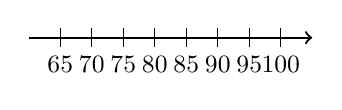
\begin{tikzpicture}[scale=0.08]
  \draw[thick,->] (60,0) -- (105,0);
  \foreach \x in {65,70,...,100} {
    \draw (\x,1.5) -- (\x,-1.5) node[below,font=\small] {$\x$};
  }
\end{tikzpicture}
\end{center}
\end{questionText}
\correctAnswer{$s \geq 87$; closed circle at $87$, shade right}
\explanation{$\frac{78 + 85 + 90 + s}{4} \geq 85$. Multiply by $4$: $253 + s \geq 340$. Subtract $253$: $s \geq 87$. Closed circle at $87$, shade right.}
\end{practiceQuestion}

\begin{practiceQuestion}{6-1-q24}{sa}
\begin{questionText}
A drawing of a room uses scale $1$ cm $= 3$ m. The drawing shows a square room with side $4$ cm. If the scale factor doubles all lengths, by what factor does the actual area change?
\end{questionText}
\correctAnswer{The area does not change}
\explanation{The actual room stays the same. Changing the drawing scale does not change the real room's area. The area of the real room is always $12 \times 12 = 144$ m$^2$.}
\end{practiceQuestion}

\begin{practiceQuestion}{6-3-q05}{mc}
\begin{questionText}
Can a triangle have sides $6$, $8$, and $14$?
\end{questionText}
\choiceA{Yes, it is a right triangle}
\choiceB{Yes, it is an obtuse triangle}
\choiceC{No, the triangle inequality is not satisfied}
\choiceD{No, because the sides are all even numbers}
\correctAnswer{C}
\explanation{$6 + 8 = 14$, which is not greater than $14$. The sum must be strictly greater, so no triangle can be formed.}
\end{practiceQuestion}

\begin{practiceQuestion}{6-4-q06}{mc}
\begin{questionText}
Two angles of a triangle are $35°$ and $75°$. What is the third angle?
\end{questionText}
\choiceA{$60°$}
\choiceB{$70°$}
\choiceC{$80°$}
\choiceD{$110°$}
\correctAnswer{B}
\explanation{$180° - 35° - 75° = 70°$.}
\end{practiceQuestion}

\begin{practiceQuestion}{6-5-q06}{mc}
\begin{questionText}
You slice a cube with a vertical cut from one face to the opposite face, perpendicular to the base. What is the most likely cross-section shape?
\end{questionText}
\choiceA{Square or rectangle}
\choiceB{Circle}
\choiceC{Triangle}
\choiceD{Hexagon}
\correctAnswer{A}
\explanation{A vertical cut through a cube perpendicular to the base typically produces a rectangle. If the cut goes through the center parallel to a face, it can be a square.}
\end{practiceQuestion}

\begin{practiceQuestion}{6-6-q10}{mc}
\begin{questionText}
Two angles are supplementary. One is $25°$ more than the other. What are the two angles?
\end{questionText}
\choiceA{$65°$ and $115°$}
\choiceB{$77.5°$ and $102.5°$}
\choiceC{$80°$ and $100°$}
\choiceD{$75°$ and $105°$}
\correctAnswer{B}
\explanation{Let the smaller be $x$. Then $x + (x + 25) = 180$. Combine: $2x + 25 = 180$. Solve: $2x = 155$, $x = 77.5°$. The other: $77.5 + 25 = 102.5°$.}
\end{practiceQuestion}

\begin{practiceQuestion}{6-7-q20}{sa}
\begin{questionText}
Reflect point $P(-6, 2)$ over the $x$-axis. What are the coordinates of $P'$?
\end{questionText}
\correctAnswer{$P'(-6, -2)$}
\explanation{Over the $x$-axis: keep $x$, negate $y$. $(-6, 2) \to (-6, -2)$.}
\end{practiceQuestion}

\begin{practiceQuestion}{7-3-q04}{mc}
\begin{questionText}
A circle has an area of $78.5$ cm$^2$. Using $\pi \approx 3.14$, what is the radius?
\end{questionText}
\choiceA{$4$ cm}
\choiceB{$5$ cm}
\choiceC{$10$ cm}
\choiceD{$25$ cm}
\correctAnswer{B}
\explanation{$r^2 = A \div \pi = 78.5 \div 3.14 = 25$. So $r = 5$ cm.}
\end{practiceQuestion}

\begin{practiceQuestion}{7-4-q17}{mc}
\begin{questionText}
A swimming pool is shaped like a rectangle $25$ m by $10$ m with a semicircle of diameter $10$ m at one end. What is the total area? Use $\pi \approx 3.14$.
\end{questionText}
\choiceA{$250$ m$^2$}
\choiceB{$289.25$ m$^2$}
\choiceC{$328.5$ m$^2$}
\choiceD{$367.75$ m$^2$}
\correctAnswer{B}
\explanation{Rectangle: $25 \times 10 = 250$ m$^2$. Semicircle: $\frac{1}{2} \times 3.14 \times 5^2 = \frac{1}{2} \times 78.5 = 39.25$ m$^2$. Total: $250 + 39.25 = 289.25$ m$^2$.}
\end{practiceQuestion}

\begin{practiceQuestion}{7-5-q24}{sa}
\begin{questionText}
A triangular prism has a right-triangle base with legs $3$ cm and $4$ cm. The prism is $12$ cm long. The hypotenuse of the triangle is $5$ cm. What is the total surface area?
\end{questionText}
\correctAnswer{$156$ cm$^2$}
\explanation{Two triangles: $2 \times \frac{1}{2} \times 3 \times 4 = 12$ cm$^2$. Three rectangles: $3 \times 12 + 4 \times 12 + 5 \times 12 = 36 + 48 + 60 = 144$ cm$^2$. Total: $12 + 144 = 156$ cm$^2$.}
\end{practiceQuestion}

\begin{practiceQuestion}{7-6-q05}{mc}
\begin{questionText}
A triangular prism has a base that is a triangle with base $8$ cm and height $3$ cm. The prism is $10$ cm long. What is the volume?
\end{questionText}
\choiceA{$24$ cm$^3$}
\choiceB{$80$ cm$^3$}
\choiceC{$120$ cm$^3$}
\choiceD{$240$ cm$^3$}
\correctAnswer{C}
\explanation{$B = \frac{1}{2} \times 8 \times 3 = 12$ cm$^2$. $V = Bh = 12 \times 10 = 120$ cm$^3$.}
\end{practiceQuestion}

\begin{practiceQuestion}{8-1-q25}{sa}
\begin{questionText}
A factory produces $10{,}000$ batteries per day. A sample of $200$ batteries is tested, and $8$ are defective. What percent of the sample is defective?
\end{questionText}
\correctAnswer{$4\%$}
\explanation{$\frac{8}{200} = 0.04 = 4\%$.}
\end{practiceQuestion}

\begin{practiceQuestion}{8-3-q27}{gmc}
\begin{questionText}
The dot plots below show the number of push-ups completed by students in two gym classes.

\begin{center}
\begin{tikzpicture}[scale=0.55]
  % Class 1
  \node[left,font=\small\bfseries] at (4,2.5) {Class 1};
  \draw[thick,->] (4.5,0) -- (16.5,0);
  \foreach \x in {5,6,...,16} {
    \draw (\x,0.1) -- (\x,-0.1);
    \node[below,font=\tiny] at (\x,0) {$\x$};
  }
  % Class 1 data: 7(1),8(2),9(3),10(4),11(3),12(2),13(1)
  \fill[funBlue] (7,0.4) circle (0.15);
  \fill[funBlue] (8,0.4) circle (0.15); \fill[funBlue] (8,0.75) circle (0.15);
  \fill[funBlue] (9,0.4) circle (0.15); \fill[funBlue] (9,0.75) circle (0.15); \fill[funBlue] (9,1.1) circle (0.15);
  \fill[funBlue] (10,0.4) circle (0.15); \fill[funBlue] (10,0.75) circle (0.15); \fill[funBlue] (10,1.1) circle (0.15); \fill[funBlue] (10,1.45) circle (0.15);
  \fill[funBlue] (11,0.4) circle (0.15); \fill[funBlue] (11,0.75) circle (0.15); \fill[funBlue] (11,1.1) circle (0.15);
  \fill[funBlue] (12,0.4) circle (0.15); \fill[funBlue] (12,0.75) circle (0.15);
  \fill[funBlue] (13,0.4) circle (0.15);

  % Class 2
  \node[left,font=\small\bfseries] at (4,5.5) {Class 2};
  \draw[thick,->] (4.5,3.5) -- (16.5,3.5);
  \foreach \x in {5,6,...,16} {
    \draw (\x,3.6) -- (\x,3.4);
    \node[below,font=\tiny] at (\x,3.4) {};
  }
  % Class 2 data: 10(1),11(2),12(3),13(4),14(3),15(2),16(1)
  \fill[funGreen] (10,3.9) circle (0.15);
  \fill[funGreen] (11,3.9) circle (0.15); \fill[funGreen] (11,4.25) circle (0.15);
  \fill[funGreen] (12,3.9) circle (0.15); \fill[funGreen] (12,4.25) circle (0.15); \fill[funGreen] (12,4.6) circle (0.15);
  \fill[funGreen] (13,3.9) circle (0.15); \fill[funGreen] (13,4.25) circle (0.15); \fill[funGreen] (13,4.6) circle (0.15); \fill[funGreen] (13,4.95) circle (0.15);
  \fill[funGreen] (14,3.9) circle (0.15); \fill[funGreen] (14,4.25) circle (0.15); \fill[funGreen] (14,4.6) circle (0.15);
  \fill[funGreen] (15,3.9) circle (0.15); \fill[funGreen] (15,4.25) circle (0.15);
  \fill[funGreen] (16,3.9) circle (0.15);
\end{tikzpicture}
\end{center}

Which class has a higher center, and by approximately how many push-ups?
\end{questionText}
\choiceA{Class 1, by about $3$}
\choiceB{Class 2, by about $3$}
\choiceC{Class 2, by about $6$}
\choiceD{They have the same center}
\correctAnswer{B}
\explanation{Class 1 center $\approx 10$. Class 2 center $\approx 13$. Difference $\approx 3$ push-ups. Class 2 is higher.}
\end{practiceQuestion}

\begin{practiceQuestion}{8-4-q29}{gsa}
\begin{questionText}
The dot plots show daily high temperatures (°F) for two cities over $10$ days.

\begin{center}
\begin{tikzpicture}[scale=0.45]
  % City A
  \node[left,font=\small\bfseries] at (57,2) {City A};
  \draw[thick,->] (57,0) -- (77,0);
  \foreach \x in {58,60,...,76} {
    \draw (\x,0.15) -- (\x,-0.15);
    \node[below,font=\tiny] at (\x,0) {$\x$};
  }
  % City A: 62,64,64,66,66,66,68,68,70,72  mean=66.6
  \fill[funBlue] (62,0.4) circle (0.18);
  \fill[funBlue] (64,0.4) circle (0.18); \fill[funBlue] (64,0.8) circle (0.18);
  \fill[funBlue] (66,0.4) circle (0.18); \fill[funBlue] (66,0.8) circle (0.18); \fill[funBlue] (66,1.2) circle (0.18);
  \fill[funBlue] (68,0.4) circle (0.18); \fill[funBlue] (68,0.8) circle (0.18);
  \fill[funBlue] (70,0.4) circle (0.18);
  \fill[funBlue] (72,0.4) circle (0.18);

  % City B
  \node[left,font=\small\bfseries] at (57,5.5) {City B};
  \draw[thick,->] (57,3.5) -- (77,3.5);
  \foreach \x in {58,60,...,76} {
    \draw (\x,3.65) -- (\x,3.35);
  }
  % City B: 58,60,64,66,68,70,72,74,74,76  mean=68.2
  \fill[funOrange] (58,3.9) circle (0.18);
  \fill[funOrange] (60,3.9) circle (0.18);
  \fill[funOrange] (64,3.9) circle (0.18);
  \fill[funOrange] (66,3.9) circle (0.18);
  \fill[funOrange] (68,3.9) circle (0.18);
  \fill[funOrange] (70,3.9) circle (0.18);
  \fill[funOrange] (72,3.9) circle (0.18);
  \fill[funOrange] (74,3.9) circle (0.18); \fill[funOrange] (74,4.3) circle (0.18);
  \fill[funOrange] (76,3.9) circle (0.18);
\end{tikzpicture}
\end{center}

Find the mean and range for each city. Which city has more consistent temperatures?
\end{questionText}
\correctAnswer{City A: mean $= 66.6$°F, range $= 10$°F. City B: mean $= 68.2$°F, range $= 18$°F. City A is more consistent.}
\explanation{City A: $(62+64+64+66+66+66+68+68+70+72) \div 10 = 666 \div 10 = 66.6$. Range $= 72 - 62 = 10$. City B: $(58+60+64+66+68+70+72+74+74+76) \div 10 = 682 \div 10 = 68.2$. Range $= 76 - 58 = 18$. City A has the smaller range.}
\end{practiceQuestion}

\begin{practiceQuestion}{8-7-q01}{mc}
\begin{questionText}
A frequency table lists:
\end{questionText}
\choiceA{Only the largest and smallest values}
\choiceB{Categories and how often each occurs}
\choiceC{The mean, median, and mode}
\choiceD{Data arranged in a circle}
\correctAnswer{B}
\explanation{A frequency table shows each category (or interval) and the count of data values in it.}
\end{practiceQuestion}

\begin{practiceQuestion}{9-4-q14}{mc}
\begin{questionText}
A student creates a probability model for a spinner: $P(\text{red}) = 0.25$, $P(\text{blue}) = 0.25$, $P(\text{green}) = 0.25$, $P(\text{yellow}) = 0.25$. After $200$ spins, the results are: red $= 55$, blue $= 48$, green $= 52$, yellow $= 45$. Is the model a good fit?
\end{questionText}
\choiceA{No, the model is completely wrong}
\choiceB{Yes, the observed frequencies are reasonably close to $50$ each}
\choiceC{No, because the results are not exactly $50$ each}
\choiceD{Yes, because $200$ is divisible by $4$}
\correctAnswer{B}
\explanation{Each color should appear about $50$ times ($200 \times 0.25$). The results ($55, 48, 52, 45$) are all close to $50$, supporting the model.}
\end{practiceQuestion}

\begin{practiceQuestion}{9-6-q27}{gmc}
\begin{questionText}
The tree diagram shows the outcomes for flipping two coins. What is the probability of getting at least one tail?

\begin{center}
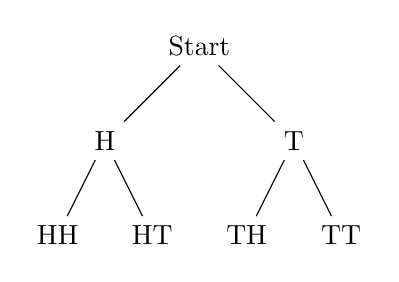
\begin{tikzpicture}[scale=0.8,
  level 1/.style={sibling distance=3cm, level distance=1.5cm},
  level 2/.style={sibling distance=1.5cm, level distance=1.5cm}]
  \node {Start}
    child {node {H}
      child {node {HH}}
      child {node {HT}}
    }
    child {node {T}
      child {node {TH}}
      child {node {TT}}
    };
\end{tikzpicture}
\end{center}
\end{questionText}
\choiceA{$\frac{1}{4}$}
\choiceB{$\frac{1}{2}$}
\choiceC{$\frac{3}{4}$}
\choiceD{$\frac{2}{4}$}
\correctAnswer{C}
\explanation{Outcomes with at least one tail: HT, TH, TT — that is $3$ out of $4$. $P = \frac{3}{4}$.}
\end{practiceQuestion}

\begin{practiceQuestion}{9-7-q27}{gmc}
\begin{questionText}
The bar graph shows the results of simulating a spinner $100$ times. The spinner is supposed to land on each color with equal probability. Based on the simulation, does the spinner appear fair?

\begin{center}
\begin{tikzpicture}[scale=0.55]
  \draw[thick,->] (0,0) -- (0,32) node[above,font=\small] {Frequency};
  \draw[thick,->] (0,0) -- (7,0);
  \foreach \y in {5,10,...,30} {
    \draw[gray!30] (0,\y) -- (6.5,\y);
    \node[left,font=\small] at (0,\y) {\y};
  }
  \fill[funRed!70] (0.5,0) rectangle (1.5,26);
  \fill[funBlue!70] (2.5,0) rectangle (3.5,24);
  \fill[funGreen!70] (4.5,0) rectangle (5.5,28);
  \node[below,font=\small] at (1,0) {Red};
  \node[below,font=\small] at (3,0) {Blue};
  \node[below,font=\small] at (5,0) {Grn.};
  \node[below,font=\small] at (3,-1) {Not shown: Yellow $= 22$};
\end{tikzpicture}
\end{center}
\end{questionText}
\choiceA{No, because the bars are different heights}
\choiceB{Yes, the frequencies ($26, 24, 28, 22$) are all roughly close to $25$}
\choiceC{No, Green is clearly the most likely color}
\choiceD{Cannot be determined from the graph}
\correctAnswer{B}
\explanation{With $4$ equal sections, each should appear about $25$ times in $100$ spins. The results ($26, 24, 28, 22$) are all close to $25$, suggesting the spinner is fair.}
\end{practiceQuestion}
